\documentclass[12pt,norsk,a4paper]{report}
\pdfobjcompresslevel=0
\usepackage[usenames,dvipsnames]{xcolor}
\usepackage[includeheadfoot,margin=0.8 in,top=0.6 in]{geometry}
\usepackage{siunitx,physics,cancel,upgreek,varioref,minted,booktabs,tocloft, pdfpages}
\usepackage{mathtools}
\usepackage{babel}
\usepackage{graphicx}
\usepackage{float}
\usepackage{fouriernc}
\usepackage{fancyhdr}
\usepackage[utf8]{inputenc}
\usepackage{amsmath}
\usepackage{amssymb}
\usepackage{textcomp}
\usepackage{lastpage}
\usepackage{microtype}
\usepackage[linktoc=all, bookmarks=true, pdfauthor={Anders Johansson}]{hyperref}
\renewcommand{\CancelColor}{\color{red}}
\renewcommand{\exp}[1]{\mathrm{e}^{#1}}
\newcommand{\tittel}[1]{\title{#1 \vspace{-7ex}}\author{}\date{}\maketitle\thispagestyle{fancy}\pagestyle{fancy}\setcounter{page}{1}}

\newcommand{\deloppg}[2][]{\subsection*{#2) #1}\addcontentsline{toc}{subsection}{#2)}\refstepcounter{subsection}\label{#2}}
\newcommand{\oppg}[1]{\section*{Oppgave #1}\addcontentsline{toc}{section}{Oppgave #1}\refstepcounter{section}\label{oppg#1}}

\labelformat{section}{seksjon~#1}
\labelformat{subsection}{avsnitt~#1}
\labelformat{subsubsection}{avsnitt~#1}
\labelformat{equation}{likning~(#1)}
\labelformat{figure}{figur~#1}
\labelformat{table}{tabell~#1}

\renewcommand{\footrulewidth}{\headrulewidth}
\tocloftpagestyle{fancy}

\setcounter{secnumdepth}{4}
\renewcommand{\thesection}{\arabic{section}}
\renewcommand{\thesubsection}{\arabic{section}.\arabic{subsection}}
\renewcommand{\thesubsubsection}{\arabic{section}.\arabic{subsection}.\arabic{subsubsection}}
\setlength{\parindent}{0cm}
\setlength{\parskip}{1em}

\newcommand{\eqtag}[1]{\refstepcounter{equation}\tag{\theequation}\label{#1}}
\hypersetup{colorlinks=true,urlcolor=blue,linkcolor=black}

\sisetup{detect-all}
\sisetup{exponent-product = \cdot, output-product = \cdot,per-mode=symbol}
\sisetup{output-decimal-marker={,}}
\sisetup{round-mode = off, round-precision=3}
\sisetup{number-unit-product = \ }

\allowdisplaybreaks[4]
\fancyhf{}

\rhead{Anders Johansson}
\rfoot{Side \thepage{} av \pageref{LastPage}}
\lhead{FYS3150}
%
\usepackage[backend=biber,citestyle=numeric-comp,bibstyle=numeric,sorting=none]{biblatex}
\DefineBibliographyStrings{norsk}{%
  bibliography = {Referanser},
}
\addbibresource{kilder.bib}

\begin{document}
%
\includepdf{forside.pdf}
\pagestyle{fancy}
\tableofcontents

\section{Sammendrag}

Alle filene til dette prosjektet finnes på GitHub\footnote{\url{https://github.com/anjohan/Offentlig/tree/master/FYS3150/Oblig2}}.


\section{Introduksjon}
Differensiallikninger er en sentral del av fysikken, ettersom mange av de mest sentrale lovene og likningene (f.eks. Newtons lover og Schrödingerlikningen) er differensiallikninger. Majoriteten av disse likningene er vanskelige eller umulige å løse analytisk, så numeriske løsningsmetoder for differensiallikninger er et viktig verktøy for fysikere.

\section{Obligbesvarelse}
\deloppg{a}
Hvis \(U\) er ortogonal, er \(U^TU=I\). Dette gir:
\[
\vec{w}_i^T\vec{w}_j = \qty(U\vec{v}_i)^T\qty(U\vec{v}_j) = \vec{v}_i^T\overbrace{U^TU}^I\vec{v}_j = \vec{v}_i^T\vec{v}_j=\vec{v}_i\cdot \vec{v}_j
\]
Ortogonale transformasjoner bevarer altså prikkproduktet, og dermed også ortogonaliteten.


\begin{figure}[H]
\centering
% GNUPLOT: LaTeX picture with Postscript
\begingroup
  \makeatletter
  \providecommand\color[2][]{%
    \GenericError{(gnuplot) \space\space\space\@spaces}{%
      Package color not loaded in conjunction with
      terminal option `colourtext'%
    }{See the gnuplot documentation for explanation.%
    }{Either use 'blacktext' in gnuplot or load the package
      color.sty in LaTeX.}%
    \renewcommand\color[2][]{}%
  }%
  \providecommand\includegraphics[2][]{%
    \GenericError{(gnuplot) \space\space\space\@spaces}{%
      Package graphicx or graphics not loaded%
    }{See the gnuplot documentation for explanation.%
    }{The gnuplot epslatex terminal needs graphicx.sty or graphics.sty.}%
    \renewcommand\includegraphics[2][]{}%
  }%
  \providecommand\rotatebox[2]{#2}%
  \@ifundefined{ifGPcolor}{%
    \newif\ifGPcolor
    \GPcolortrue
  }{}%
  \@ifundefined{ifGPblacktext}{%
    \newif\ifGPblacktext
    \GPblacktextfalse
  }{}%
  % define a \g@addto@macro without @ in the name:
  \let\gplgaddtomacro\g@addto@macro
  % define empty templates for all commands taking text:
  \gdef\gplbacktext{}%
  \gdef\gplfronttext{}%
  \makeatother
  \ifGPblacktext
    % no textcolor at all
    \def\colorrgb#1{}%
    \def\colorgray#1{}%
  \else
    % gray or color?
    \ifGPcolor
      \def\colorrgb#1{\color[rgb]{#1}}%
      \def\colorgray#1{\color[gray]{#1}}%
      \expandafter\def\csname LTw\endcsname{\color{white}}%
      \expandafter\def\csname LTb\endcsname{\color{black}}%
      \expandafter\def\csname LTa\endcsname{\color{black}}%
      \expandafter\def\csname LT0\endcsname{\color[rgb]{1,0,0}}%
      \expandafter\def\csname LT1\endcsname{\color[rgb]{0,1,0}}%
      \expandafter\def\csname LT2\endcsname{\color[rgb]{0,0,1}}%
      \expandafter\def\csname LT3\endcsname{\color[rgb]{1,0,1}}%
      \expandafter\def\csname LT4\endcsname{\color[rgb]{0,1,1}}%
      \expandafter\def\csname LT5\endcsname{\color[rgb]{1,1,0}}%
      \expandafter\def\csname LT6\endcsname{\color[rgb]{0,0,0}}%
      \expandafter\def\csname LT7\endcsname{\color[rgb]{1,0.3,0}}%
      \expandafter\def\csname LT8\endcsname{\color[rgb]{0.5,0.5,0.5}}%
    \else
      % gray
      \def\colorrgb#1{\color{black}}%
      \def\colorgray#1{\color[gray]{#1}}%
      \expandafter\def\csname LTw\endcsname{\color{white}}%
      \expandafter\def\csname LTb\endcsname{\color{black}}%
      \expandafter\def\csname LTa\endcsname{\color{black}}%
      \expandafter\def\csname LT0\endcsname{\color{black}}%
      \expandafter\def\csname LT1\endcsname{\color{black}}%
      \expandafter\def\csname LT2\endcsname{\color{black}}%
      \expandafter\def\csname LT3\endcsname{\color{black}}%
      \expandafter\def\csname LT4\endcsname{\color{black}}%
      \expandafter\def\csname LT5\endcsname{\color{black}}%
      \expandafter\def\csname LT6\endcsname{\color{black}}%
      \expandafter\def\csname LT7\endcsname{\color{black}}%
      \expandafter\def\csname LT8\endcsname{\color{black}}%
    \fi
  \fi
    \setlength{\unitlength}{0.0500bp}%
    \ifx\gptboxheight\undefined%
      \newlength{\gptboxheight}%
      \newlength{\gptboxwidth}%
      \newsavebox{\gptboxtext}%
    \fi%
    \setlength{\fboxrule}{0.5pt}%
    \setlength{\fboxsep}{1pt}%
\begin{picture}(7200.00,4320.00)%
    \gplgaddtomacro\gplbacktext{%
      \csname LTb\endcsname%
      \put(858,440){\makebox(0,0)[r]{\strut{}$-0${,}$2$}}%
      \csname LTb\endcsname%
      \put(858,956){\makebox(0,0)[r]{\strut{}$-0${,}$15$}}%
      \csname LTb\endcsname%
      \put(858,1473){\makebox(0,0)[r]{\strut{}$-0${,}$1$}}%
      \csname LTb\endcsname%
      \put(858,1989){\makebox(0,0)[r]{\strut{}$-0${,}$05$}}%
      \csname LTb\endcsname%
      \put(858,2506){\makebox(0,0)[r]{\strut{}$0$}}%
      \csname LTb\endcsname%
      \put(858,3022){\makebox(0,0)[r]{\strut{}$0${,}$05$}}%
      \csname LTb\endcsname%
      \put(858,3539){\makebox(0,0)[r]{\strut{}$0${,}$1$}}%
      \csname LTb\endcsname%
      \put(858,4055){\makebox(0,0)[r]{\strut{}$0${,}$15$}}%
      \csname LTb\endcsname%
      \put(990,220){\makebox(0,0){\strut{}$0$}}%
      \csname LTb\endcsname%
      \put(1636,220){\makebox(0,0){\strut{}$1$}}%
      \csname LTb\endcsname%
      \put(2282,220){\makebox(0,0){\strut{}$2$}}%
      \csname LTb\endcsname%
      \put(2928,220){\makebox(0,0){\strut{}$3$}}%
      \csname LTb\endcsname%
      \put(3574,220){\makebox(0,0){\strut{}$4$}}%
      \csname LTb\endcsname%
      \put(4219,220){\makebox(0,0){\strut{}$5$}}%
      \csname LTb\endcsname%
      \put(4865,220){\makebox(0,0){\strut{}$6$}}%
      \csname LTb\endcsname%
      \put(5511,220){\makebox(0,0){\strut{}$7$}}%
      \csname LTb\endcsname%
      \put(6157,220){\makebox(0,0){\strut{}$8$}}%
      \csname LTb\endcsname%
      \put(6803,220){\makebox(0,0){\strut{}$9$}}%
    }%
    \gplgaddtomacro\gplfronttext{%
      \csname LTb\endcsname%
      \put(5816,3882){\makebox(0,0)[r]{\strut{}$\lambda=3.000$}}%
      \csname LTb\endcsname%
      \put(5816,3662){\makebox(0,0)[r]{\strut{}$\lambda=6.998$}}%
      \csname LTb\endcsname%
      \put(5816,3442){\makebox(0,0)[r]{\strut{}$\lambda=10.995$}}%
    }%
    \gplbacktext
    \put(0,0){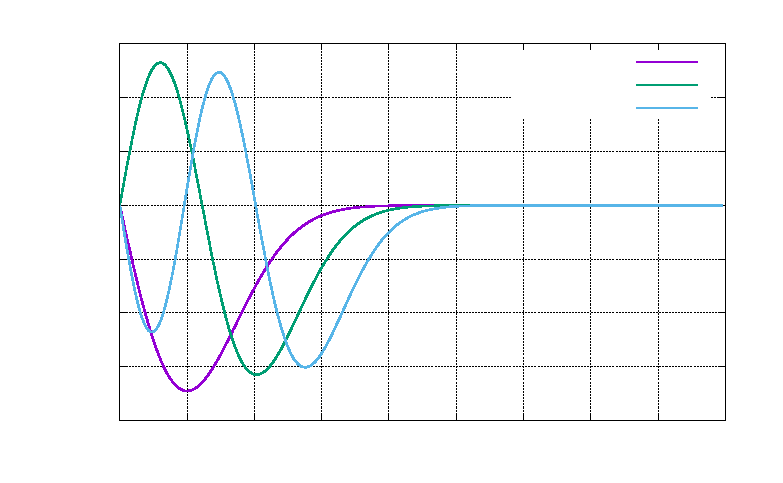
\includegraphics{plot}}%
    \gplfronttext
  \end{picture}%
\endgroup

\end{figure}














\clearpage
\addcontentsline{toc}{section}{Referanser}
\printbibliography


\end{document}
